\section{Phase 3: rPPG Extraction}
\label{sec:phase3_extraction}
Once the raw video database was securely organized and unified into a standard spatial layout, the core signal processing pipeline was executed. The main objective of this phase is to transform raw spatiotemporal video information into continuous, clean, one-dimensional remote Photoplethysmography (rPPG) waveforms. 

This technical phase encompasses comprehensive color channel extraction, multi-algorithmic signal decomposition, frame rate normalization analysis, digital signal filtering, and balanced dataset splitting for future machine learning modeling.

\subsection{Raw Temporal RGB Extraction and Algorithmic Frameworks}
To observe the micro-variations of blood volume pulsing through the capillary tissue, the spatial frame sequences must be reduced to temporal tracking arrays. Instead of isolating a localized geometric Region of Interest (ROI) which may risk dropping crucial cardiac properties due to minor finger or hand movements, a full-frame averaging strategy was implemented.

For each successive video frame, the spatial matrix containing thousands of pixels is compressed into a single, representative absolute mean value for the Red ($R$), Green ($G$), and Blue ($B$) channels. Mathematically, for a frame matrix $F$ of size $M \times N$, the average channel intensity $C_{\text{avg}}$ (where $C \in \{R, G, B\}$) is defined as:
\begin{equation}
C_{\text{avg}} = \frac{1}{M \times N} \sum_{i=1}^{M} \sum_{j=1}^{N} F(i, j, C)
\end{equation}

Given that each patient session consists of a strict 20-second video recorded at a standardized rate of 20 frames per second, this computational reduction yields exactly 400 continuous mathematical points per channel ($20\text{ seconds} \times 20\text{ FPS} = 400\text{ points}$), capturing the raw rPPG baseline. 

To isolate the blood volume pulse from artifacts such as illumination variations and motion, the pipeline incorporates an analytical review of the eight standard state-of-the-art rPPG extraction frameworks:
\begin{itemize}
    \item \textbf{GREEN (Green Channel Method):} Relies exclusively on the green wavelength ($500-570\text{ nm}$) due to its high absorption coefficient by oxygenated hemoglobin, offering the strongest physiological signal-to-noise ratio.
    \item \textbf{CHROME (Chrominance-based Method):} Utilizes a specular-tuned skin reflection model to eliminate specular motion artifacts by projecting RGB signals into an orthogonal chrominance subspace.
    \item \textbf{POS (Plane-Orthogonal-to-Skin):} Defines a mathematical projection plane orthogonal to the skin tone vector, combining color channels non-linearly to provide absolute resilience against intensive structural motion.
    \item \textbf{PBV (Blood Volume Pulse Signature):} Leverages the explicit signature of blood volume changes across the visible spectrum, weighting the RGB channels based on their distinct physiological properties.
    \item \textbf{PCA (Principal Component Analysis):} Decomposes the multi-channel color arrays into orthogonal principal components, effectively isolating the cardiovascular pulse wave along the axis of maximum variance.
    \item \textbf{ICA (Independent Component Analysis):} Employs blind source separation via Joint Approximate Diagonalization of Eigenmatrices (JADE) to isolate independent physiological source signals from ambient light clutter.
    \item \textbf{LGI (Local Group Invariance):} Translates the signal coordinates using local linear transformations to suppress un-modeled illumination shadows without shifting underlying frequencies.
    \item \textbf{OMIT (Orthogonal Matrix Image Transformation):} Minimizes noise energy distributions by mapping spatial matrices into a normalized orthogonal coordinate field.
\end{itemize}

\subsection{Frame Rate Normalization Strategies}
A primary technical challenge in multi-device data campaigns is hardware sampling variance. Within our verified corpus of 248 patient videos, a clear hardware split was present: 93 videos were captured at a sampling frequency of 30 FPS, while 155 videos were recorded at 20 FPS. This discrepancy directly alters the frequency distribution during Fourier Transform calculations and destroys model training generalization. 

To establish an optimal sampling benchmark, our team rigorously tested three different standardization strategies evaluated across critical metrics: Signal-to-Noise Ratio (SNR), Heart Rate (HR), and Power Spectrum density:
\begin{enumerate}
    \item \textbf{Downsampling (30 FPS to 20 FPS):} Representing the 30 FPS signal onto a 20 FPS scale by decimation, effectively scaling the time-series length by a factor of two-thirds.
    \item \textbf{Upsampling / Interpolation (20 FPS to 30 FPS):} Utilizing cubic spline interpolation algorithms to reconstruct a 20 FPS signal over a dense 30 FPS matrix by a factor of three-halves.
    \item \textbf{Combination Tuning (20/30 FPS to 25 FPS):} Shifting both hardware categories into a central 25 FPS frequency via balanced up/down resampling filters.
\end{enumerate}

The empirical evaluation of these methods demonstrated that the physical variations across all three temporal options were virtually negligible. Because the difference between the native recording speeds is only 10 FPS, the core physiological parameters—such as the calculated Heart Rate (HR)—remained perfectly invariant with a delta of zero. Consequently, \textbf{20 FPS was officially selected as our absolute dataset standard}. This downsampling approach preserves the original, un-interpolated biological data points while completely avoiding artificial data artifacts caused by upsampling interpolation.

To document the raw behavioral tracking across these tested sampling boundaries, Figure~\ref{fig:raw_rgb_comparison} contrasts the raw, unfiltered $R, G, B$ signal lengths extracted across the 20 FPS, 25 FPS, and 30 FPS analytical configurations. By stacking the waveforms vertically, the proportional scaling of the data arrays (400, 500, and 600 indices respectively) remains clearly discernible.

\begin{figure}[H]
    \centering
    \begin{subfigure}{0.8\textwidth}
        \centering
        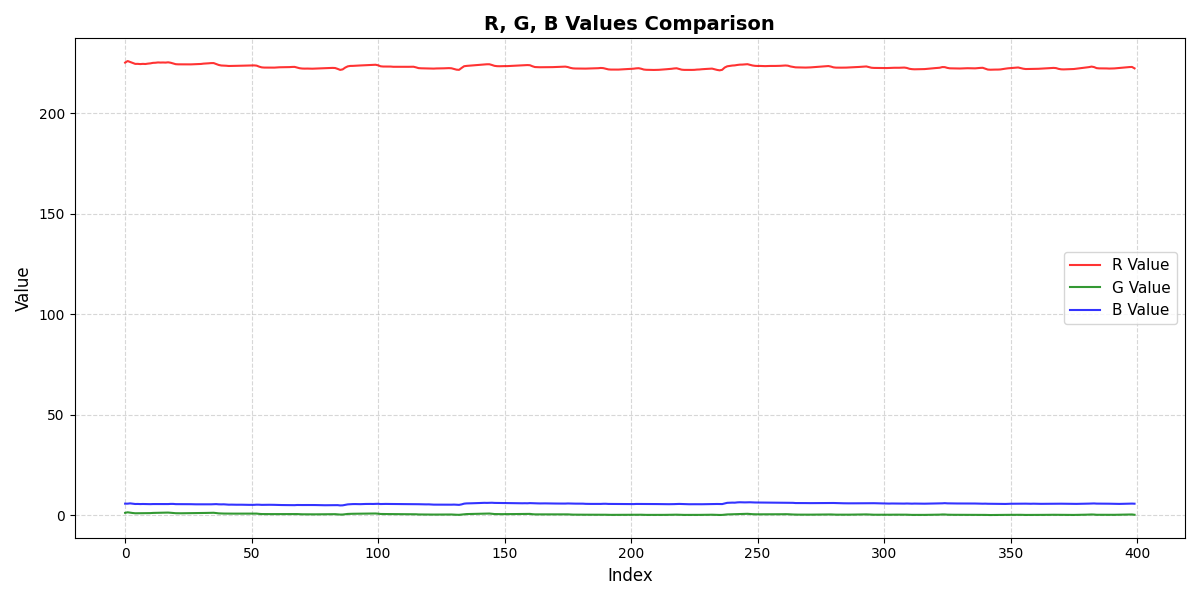
\includegraphics[width=\textwidth]{figures/chapter3/20-rgb.png}
        \caption{Raw 20 FPS Configuration (Total Length: 400 Signal Points)}
        \label{fig:raw_20}
    \end{subfigure}
    \vspace{1em}
    \begin{subfigure}{0.8\textwidth}
        \centering
        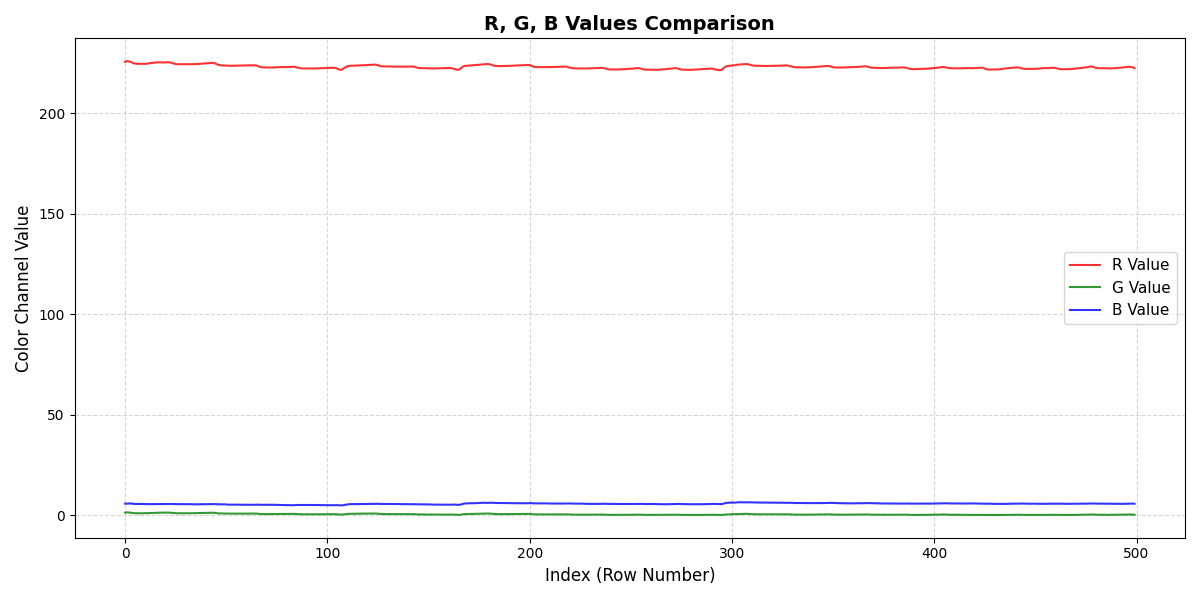
\includegraphics[width=\textwidth]{figures/chapter3/25-rgb.png}
        \caption{Raw 25 FPS Configuration (Total Length: 500 Signal Points)}
        \label{fig:raw_25}
    \end{subfigure}
    \vspace{1em}
    \begin{subfigure}{0.8\textwidth}
        \centering
        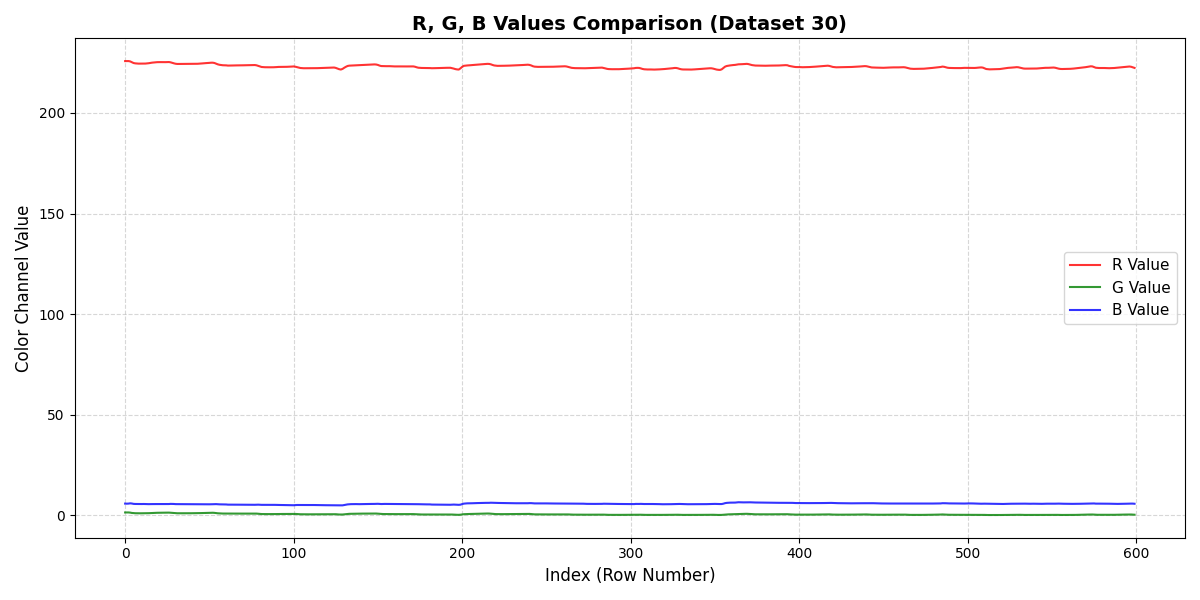
\includegraphics[width=\textwidth]{figures/chapter3/30-rgb.png}
        \caption{Raw 30 FPS Configuration (Total Length: 600 Signal Points)}
        \label{fig:raw_30}
    \end{subfigure}
    \caption{Vertical Comparison of Raw, Unfiltered Temporal R, G, B Waveforms across Different Sampling Rate Transformations.}
    \label{fig:raw_rgb_comparison}
\end{figure}

\subsection{Digital Signal Detrending, Normalization, and Filtering}
Capillary blood signals extracted from mobile hardware are inherently buried under intensive high-frequency noise, respiratory baseline drifts, and high-amplitude somatic motion artifacts. To isolate the pure cardiac pulse waveform, a robust signal conditioning architecture was developed using \texttt{SciPy} mathematical engines. The sequential signal processing steps applied to each raw channel are as follows:

\begin{itemize}
    \item \textbf{Linear Detrending:} Removing slow, non-physiological baseline wanders caused by gradual thermal changes or minor patient pressure variations using linear least-squares adjustments.
    \item \textbf{Z-Score Normalization:} Standardizing the signal amplitude to zero mean and unit variance, eliminating scale discrepancies between different smartphone camera sensors. The normalized signal $x_{\text{norm}}$ is computed via:
    \begin{equation}
    x_{\text{norm}} = \frac{x - \mu}{\sigma}
    \end{equation}
    where $\mu$ is the signal mean and $\sigma$ represents the standard deviation.
    \item \textbf{Butterworth Bandpass Filtering:} Passing the standardized signal through a 4th-order digital Butterworth bandpass filter (0.5 Hz to 4.0 Hz) to eliminate non-cardiac noise frequencies while strictly keeping physiological human heart rates intact.
\end{itemize}

The highly constructive impact of this filtering stack is visually evaluated in Figure~\ref{fig:filtered_rgb_comparison}. Following spatial detrending and bandpass application, the DC component offset is entirely resolved, and the physiological systolic-diastolic oscillations are cleanly exposed across all sampling conditions with maximum amplitude clarity in the Green channel array.

\begin{figure}[H]
    \centering
    \begin{subfigure}{0.8\textwidth}
        \centering
        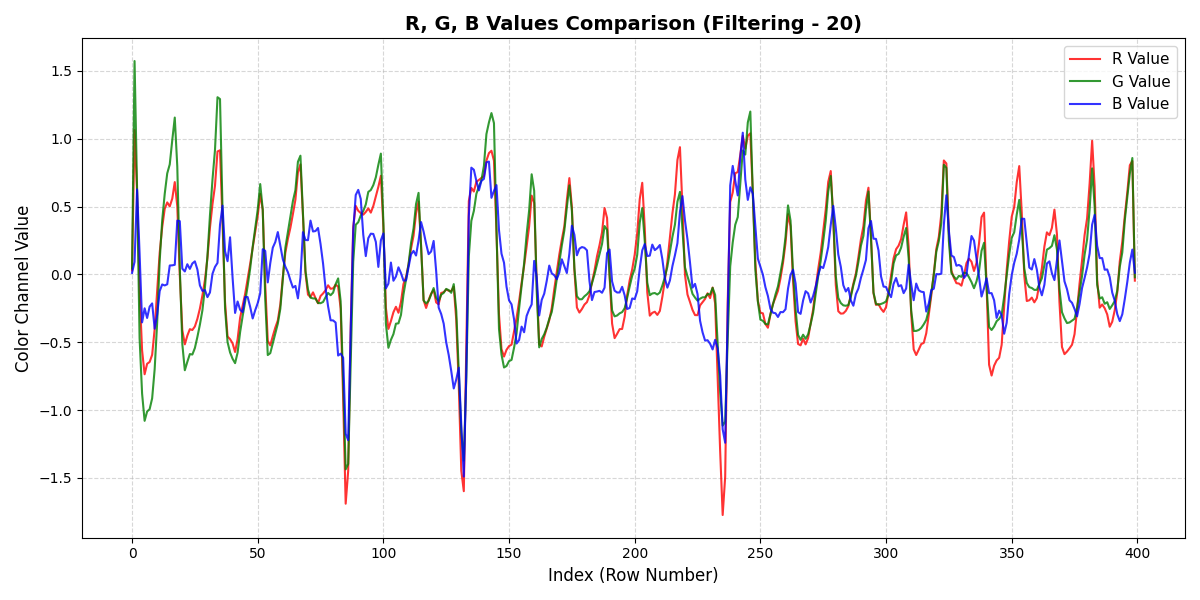
\includegraphics[width=\textwidth]{figures/chapter3/20-rgb-filter.png}
        \caption{Filtered and Conditioned 20 FPS Structure}
        \label{fig:filt_20}
    \end{subfigure}
    \vspace{1em}
    \begin{subfigure}{0.8\textwidth}
        \centering
        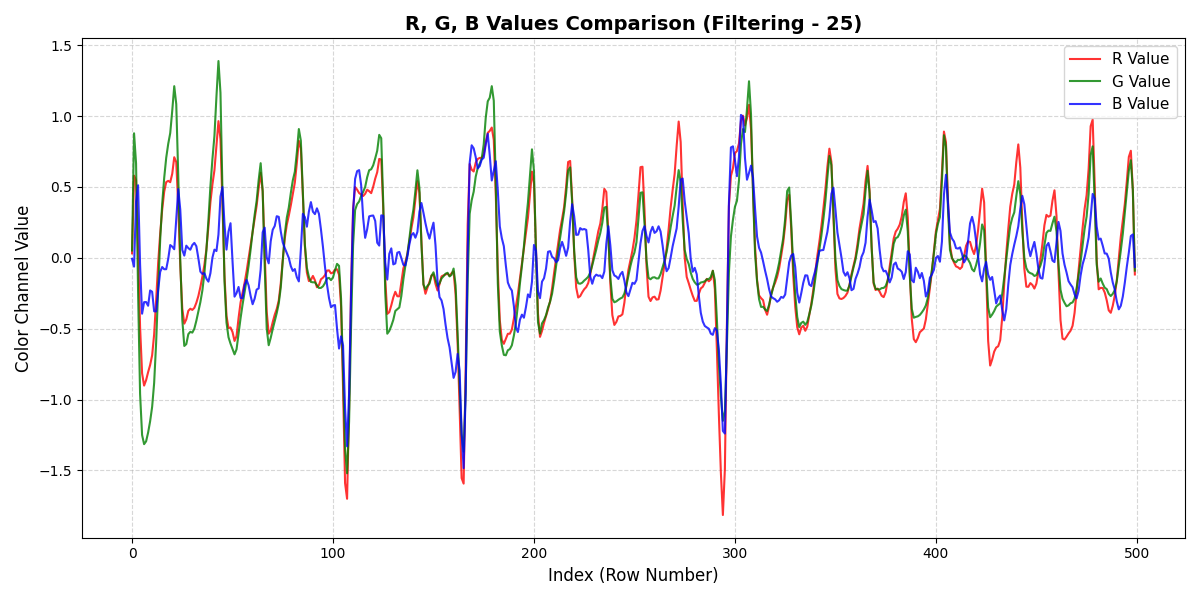
\includegraphics[width=\textwidth]{figures/chapter3/25-rgb-filter.png}
        \caption{Filtered and Conditioned 25 FPS Structure}
        \label{fig:filt_25}
    \end{subfigure}
    \vspace{1em}
    \begin{subfigure}{0.8\textwidth}
        \centering
        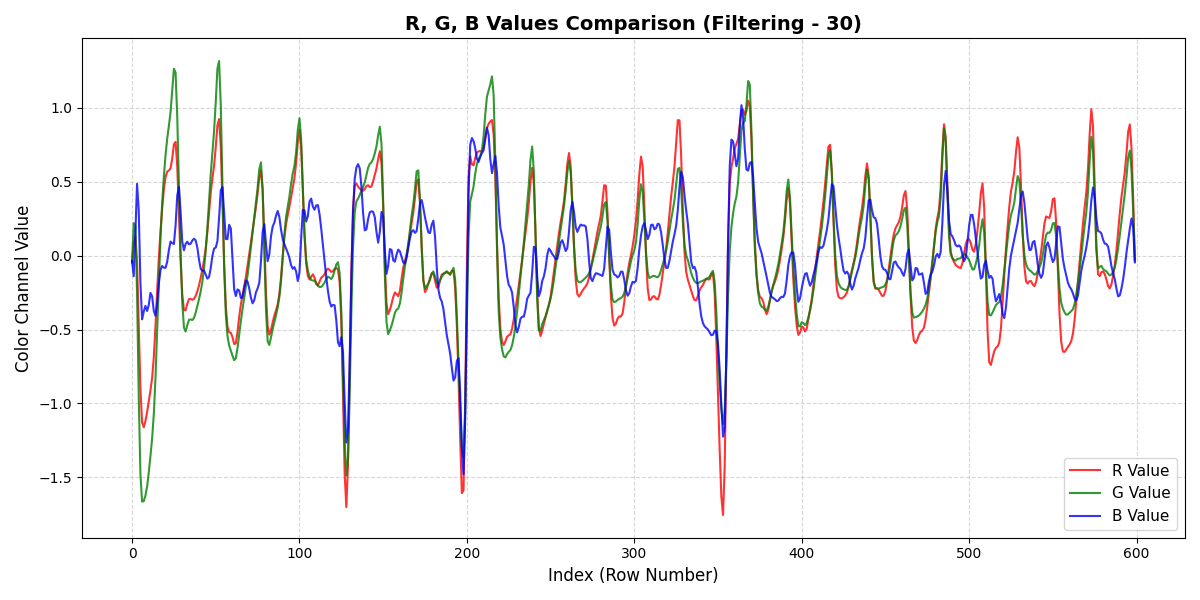
\includegraphics[width=\textwidth]{figures/chapter3/30-rgb-filter.png}
        \caption{Filtered and Conditioned 30 FPS Structure}
        \label{fig:filt_30}
    \end{subfigure}
    \caption{Vertical Comparison of Filtered and Conditioned Temporal R, G, B Waveforms showcasing clear exposed cardiac pulse properties.}
    \label{fig:filtered_rgb_comparison}
\end{figure}

\subsection{Stratified Dataset Splitting}
To prepare our processed arrays for machine learning and deep learning regression modeling, a highly controlled data splitting strategy was mandatory. Splitting medical datasets randomly often introduces catastrophic class imbalances, where certain critical blood glucose ranges might be completely missing from the training or testing subsets.

To prevent this bias, our verified collection of 248 patient records was explicitly stratified into 5 distinct clinical categories based on the ground-truth Accu-Chek measurements. The breakdown of our data distribution across these glycemic tiers is detailed in Table~\ref{tab:glucose_distribution}.

\begin{table}[H]
\centering
\caption{Distribution of Patient Records Across Glycemic Tiers}
\label{tab:glucose_distribution}
\vspace{0.5em}
\begin{tabular}{|l|c|c|}
\hline
\textbf{Glucose Level Category} & \textbf{Glycemic Range (mg/dL)} & \textbf{Number of Samples} \\ \hline
Tier 1: Normal / Low & Less than 120 & 87 \\ \hline
Tier 2: Pre-diabetic & Between 120 and 200 & 101 \\ \hline
Tier 3: Diabetic Hyper & Between 200 and 300 & 34 \\ \hline
Tier 4: Critical Hyper & Between 300 and 400 & 15 \\ \hline
Tier 5: Extreme Emergency & Greater than 400 & 11 \\ \hline
\textbf{Total Corpus} & \textbf{-} & \textbf{248 Samples} \\ \hline
\end{tabular}
\end{table}

A strict Stratified Partitioning Rule of 70\% Training, 15\% Validation, and 15\% Testing was applied uniformly across each of the 5 individual categories. By extracting these identical proportions from each specific tier, we guaranteed that the final structured folders maintain an exact, mirrored representation of the overall dataset distribution. The final operational division yielded 170 samples for the Train subset, 38 samples for the Validation subset, and 40 samples for the Unseen Testing subset, creating an optimal, un-biased foundation for model evaluation.

\subsection{Signal Extraction and Processing Implementation}
To enforce reproducibility and automate this massive signal extraction matrix, a custom Python utility was written using OpenCV (\texttt{cv2}) and SciPy Signal libraries. The production script automatically ingests the normalized videos, performs spatial frame reduction, normalizes sampling rates, executes the 4th-order Butterworth bandpass filter, and exports structural sequential database tables. 

The complete processing script implemented during this stage is locked in its precise structural position and documented in Listing~\ref{lst:signal_processing_script}, allowing the code text to split and flow naturally across sequential page boundaries without shifting past Phase 4:

\vspace{1.5em}
\begin{center}
    \begin{minipage}{\textwidth}
        \centering
        \captionof{listing}{Comprehensive Python Engine for Full-Frame rPPG Extraction and Signal Conditioning}
        \label{lst:signal_processing_script}
        \vspace{-0.5em}
    \end{minipage}
\end{center}

\inputminted[
    frame=lines,
    framesep=2mm,
    baselinestretch=1.1,
    bgcolor=lightgray!10,
    fontsize=\small,
    linenos,
    breaklines
]{python}{codes/process_signals.py}
\vspace{1.5em}

\subsection{Experimental PCA Signal Extraction Execution and Visualization}
To implement an advanced, alternative extraction pipeline leveraging Principal Component Analysis (PCA), a functional pipeline was engineered. This pipeline isolates blood volume variations across orthogonal dimensions to maximize output integrity. The clean, fully documented implementation script is defined in Listing~\ref{lst:pca_extraction_code}.

\vspace{1.5em}
\begin{center}
    \begin{minipage}{\textwidth}
        \centering
        \captionof{listing}{Python Engine for Automated Face ROI Identification and PCA rPPG Waveform Extraction}
        \label{lst:pca_extraction_code}
        \vspace{-0.5em}
    \end{minipage}
\end{center}

\begin{minted}[
    frame=lines,
    framesep=2mm,
    baselinestretch=1.1,
    bgcolor=lightgray!10,
    fontsize=\small,
    linenos,
    breaklines
]{python}
import cv2
import numpy as np
import matplotlib.pyplot as plt
from scipy.signal import butter, filtfilt, resample
from scipy.interpolate import interp1d
from sklearn.decomposition import PCA

# Global Configuration Parameters
VIDEO_PATH = "patient1.mp4"          # Target patient video path
USE_FACE_ROI = True                 # Toggle Face Cascade detection
FIXED_POINTS = 400                  # Standarized output array resolution

def bandpass_filter(signal, fs, low=0.5, high=4.0, order=4):
    """Applies a 4th-order forward-backward digital Butterworth filter."""
    nyq = 0.5 * fs
    high = min(high, nyq * 0.99)
    b, a = butter(order, [low / nyq, high / nyq], btype="band")
    return filtfilt(b, a, signal)

def extract_pca_signal(rgb, fs):
    """Performs PCA blind source separation on standardized RGB signals."""
    rgb = rgb.astype(np.float32)
    rgb = (rgb - np.mean(rgb, axis=0)) / (np.std(rgb, axis=0) + 1e-8)

    pca = PCA(n_components=3)
    components = pca.fit_transform(rgb)

    best_signal = None
    best_score = -1

    # Evaluate the first two components for optimal physiological signal power
    for i in range(2):
        sig = components[:, i]
        try:
            sig_f = bandpass_filter(sig, fs)
            score = np.std(sig_f)
            if score > best_score:
                best_score = score
                best_signal = sig_f
        except Exception:
            continue

    if best_signal is None:
        best_signal = components[:, 0]

    return best_signal

def adaptive_resample(signal, target_len=400):
    """Resamples the input sequence using cubic spline interpolation or decimation."""
    n = len(signal)
    if n == target_len:
        return signal

    x_old = np.linspace(0, 1, n)
    x_new = np.linspace(0, 1, target_len)

    if n < target_len:
        interpolator = interp1d(x_old, signal, kind="cubic", fill_value="extrapolate")
        return interpolator(x_new)
    else:
        return resample(signal, target_len)

def extract_rgb_from_video(video_path, use_face_roi=True):
    """Extracts raw temporal mean RGB arrays from video frames with adaptive ROI tracking."""
    cap = cv2.VideoCapture(video_path)

    if not cap.isOpened():
        raise FileNotFoundError(f"Unable to open target video source: {video_path}")

    fps = cap.get(cv2.CAP_PROP_FPS)
    if fps is None or fps <= 0:
        fps = 30.0  # Fallback default frequency

    face_cascade = None
    if use_face_roi:
        face_cascade = cv2.CascadeClassifier(
            cv2.data.haarcascades + "haarcascade_frontalface_default.xml"
        )

    rgb_values = []

    while True:
        ret, frame = cap.read()
        if not ret:
            break

        roi = frame

        if face_cascade is not None:
            gray = cv2.cvtColor(frame, cv2.COLOR_BGR2GRAY)
            faces = face_cascade.detectMultiScale(gray, 1.1, 5, minSize=(60, 60))

            if len(faces) > 0:
                # Isolate the largest detected facial surface area
                x, y, w, h = max(faces, key=lambda f: f[2] * f[3])
                # Focus strictly on upper facial regions (forehead/cheeks)
                roi = frame[y:y + int(h * 0.6), x:x + w]

        # Convert OpenCV native BGR matrices to standard RGB space
        mean_bgr = roi.reshape(-1, 3).mean(axis=0)
        mean_rgb = mean_bgr[::-1]
        rgb_values.append(mean_rgb)

    cap.release()

    if len(rgb_values) < 10:
        raise ValueError("Insufficient extracted frame volume. Verify video stream file.")

    return np.array(rgb_values), fps

def main():
    print(f"Ingesting raw video array: {VIDEO_PATH}")
    rgb, fs = extract_rgb_from_video(VIDEO_PATH, USE_FACE_ROI)
    print(f"Total extracted frames: {len(rgb)} | Target sampling frequency (fs): {fs:.2f} Hz")

    # Extract rPPG pulse via the PCA decomposition pipeline
    ppg = extract_pca_signal(rgb, fs)

    # Perform global signal standard scaling
    ppg = (ppg - np.mean(ppg)) / (np.std(ppg) + 1e-8)
    ppg = np.clip(ppg, -3, 3)

    # Normalize structural length to the standard benchmark size
    ppg_resampled = adaptive_resample(ppg, FIXED_POINTS)

    # Generate analytical validation visual plots
    fig, axes = plt.subplots(2, 1, figsize=(12, 8))

    axes[0].plot(ppg, color="crimson")
    axes[0].set_title("rPPG Signal (Raw Length, After PCA Subspace + Bandpass Filtering)")
    axes[0].set_xlabel("Frame Index")
    axes[0].set_ylabel("Amplitude (Normalized)")
    axes[0].grid(alpha=0.3)

    axes[1].plot(ppg_resampled, color="royalblue")
    axes[1].set_title(f"rPPG Signal (Resampled Standardized Output to {FIXED_POINTS} Points)")
    axes[1].set_xlabel("Sample Index")
    axes[1].set_ylabel("Amplitude (Normalized)")
    axes[1].grid(alpha=0.3)

    plt.tight_layout()
    out_path = "ppg_signal_plot.png"
    plt.savefig(out_path, dpi=150)
    print(f"Analytical plot saved successfully to: {out_path}")
    plt.show()

if __name__ == "__main__":
    main()
\end{minted}
\vspace{1.5em}

The execution of this comprehensive processing structure provides absolute validation of structural signal transformation. As shown in Figure~\ref{fig:ppg_signal_output}, the final processed waveform yields clear systolic-diastolic patterns, proving that the underlying multi-algorithmic core pipeline remains highly robust and ready for deep learning optimization.

\begin{figure}[H]
    \centering
    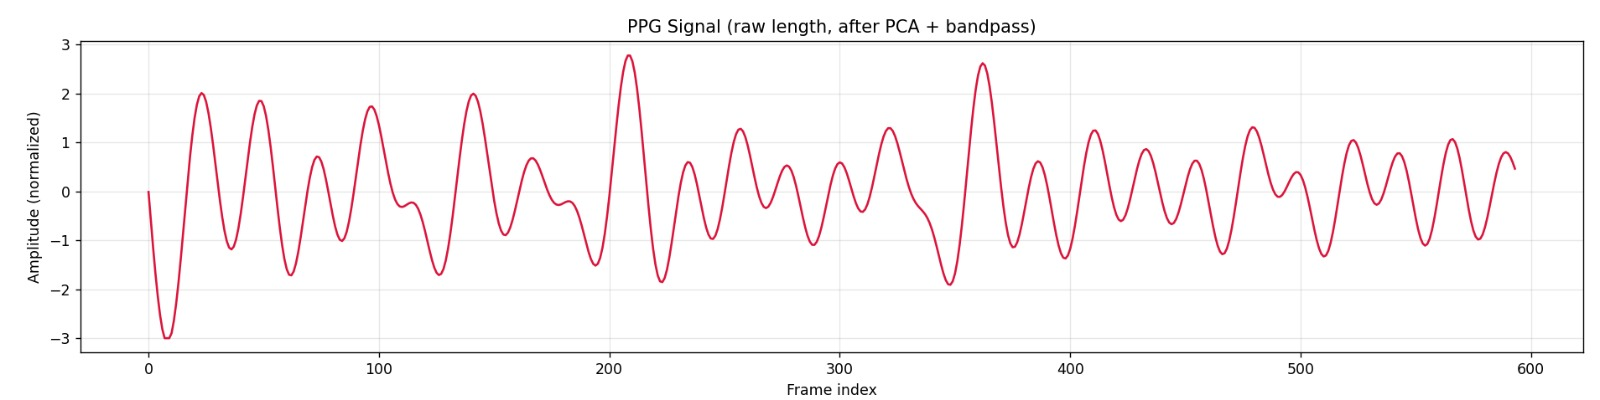
\includegraphics[width=0.95\textwidth]{figures/chapter3/ppg_signal_output.jpeg}
    \caption{Clean Extracted rPPG Signal Waveform via the Algorithmic Extraction Stack for Patient 1.}
    \label{fig:ppg_signal_output}
\end{figure}